\documentclass[9pt,twocolumn,twoside,lineno]{article}


\templatetype{article} % Choose template 
% {pnasresearcharticle} = Template for a two-column research article
% {pnasmathematics} %= Template for a one-column mathematics article
% {pnasinvited} %= Template for a PNAS invited submission

\title{The Wisdom and Manipulability of Threads}

\author[a]{Robin Engelhardt}
\author[a]{Vincent F. Hendricks} 

\affil[a]{Center for Information and Bubble Studies, Department of Media, Cognition and Communication, University of Copenhagen, Karen Blixens Plads 8, DK-2300 Copenhagen S.}
\affil[1]{ORCID: 0000-0002-7162-0990}

% Please give the surname of the lead author for the running footer
\leadauthor{Engelhardt} 

% Please add here a significance statement to explain the relevance of your work
\significancestatement{Online discussion threads are important means for individual decision-making as well as for the aggregation of collective judgments, e.g the 'wisdom of crowds’. Empirical and theoretical investigations of the wisdom of crowds are currently ambivalent about the role played by social influence. While some findings suggest that social influence undermines crowd accuracy due to correlated judgment errors, others show that accuracy improves. We demonstrate that for difficult tasks, seeing previous estimates in a thread aids individual decision-making as well as the wisdom of crowds. However, when threads are artificially filtered in such a way that participants only see the highest estimates yet made, individual accuracy as well as thread accuracy declines dramatically.}

% Please include corresponding author, author contribution and author declaration information
\authorcontributions{R. E. designed the experiment and analyzed the data, R. E. contributed as lead author, V.F.H. contributed as the co-author, V.F.H. contributed as the project manager.}
\authordeclaration{The authors declare no conflict of interest.}
\correspondingauthor{\textsuperscript{2}To whom correspondence should be addressed. E-mail: robin.engelhardt\@gmail.com}

\keywords{collective intelligence $|$ magnitude estimation $|$ decision-making $|$ discussion threads $|$  wisdom of crowds} 

\begin{abstract}
Social decision-making is increasingly relying on digitized aggregates of people’s opinions and judgments. These aggregates are frequently created and maintained as threads, i.e. as sequences of opinions on a website. While it has been shown that knowledge of thread aggregates can distort individual decision-making, it is unknown how knowledge of preceding decisions in a thread may influence collective accuracy, i.e. the wisdom of threads. We investigate experimentally the accuracy of threads in which people make magnitude estimations of varying difficulty while seeing a number of previous decisions. We find a significant increase in individual as well as collective accuracy for complex tasks. When threads are manipulated, however, individual as well as thread accuracy declines dramatically for those tasks. Our result suggests that only pristine and unfiltered threads improve individual decision-making and may be used to harness collective intelligence.
\end{abstract}

\dates{This manuscript was compiled on \today}
\doi{\url{www.pnas.org/cgi/doi/10.1073/pnas.XXXXXXXXXX}}

\begin{document}

\maketitle
\thispagestyle{firststyle}
\ifthenelse{\boolean{shortarticle}}{\ifthenelse{\boolean{singlecolumn}}{\abscontentformatted}{\abscontent}}{}

\dropcap{S}ocial information in the form of opinions and judgments by other people is sampled sequentially. We read the news, hear rumors, listen to debates on TV, and flip through comments on social media platforms and blogs. These activities inform us and influence our decisions, but researchers still debate the conditions under which these types of social information help us make better decisions \cite{woolley2010evidence, gurccay2015power, becker2017network, jayles2017social}, lead us astray \cite{caplan2011myth, lorenz2011social, minson2012cost, king2011true, le2018endogenous}, or just make us confused at a higher level \cite{salganik2006experimental, salganik2009web}. Collective estimates of a diverse group of people can outperform the majority of its members because any random confusion at the individual level is likely to average out and let the most accurate estimate prevail \cite{galton1907vox, muth1961rational, surowiecki2005wisdom, hong2008some}. Then again, confusion is not always randomly scattered around the truth. Systematic biases in individual perception may create measurable disruptions in the wisdom of crowds \cite{izard2008calibrating, nash2014curious, kao2018counteracting}. Social information can add to those biases and create cascades, echo chambers, bandwagon- and herding effects \cite{anderson1997information, bikhchandani1992theory, bakshy2015exposure, banerjee1992simple}. Partially sampled social information may lead to rich-get-richer dynamics \cite{barabasi1999emergence} and to belief misattributions, which uphold harmful social practices despite being rejected by a majority of people \cite{katz1931students, darley1968bystander, ross1977false, noelle1974spiral, lee2019homophily}. Social information may also have been intentionally filtered or manipulated in various ways, for instance through group pressure \cite{asch1951effects}, algorithmic filtering \cite{pariser2011filter}, false cues \cite{salganik2006experimental, muchnik2013social, hanson1996hits}, or simply by plain misinformation \cite{hendricks2018reality}, often with highly detrimental consequences for our economy and our health.

Observational data of decision-making processes is acutely sensitive to the social context in which people find themselves. Thus, researchers find it difficult to separate observational data into its social and individual components. How may we know how much weight an individual puts on her own ‘independent’ estimate relative to the weight put on the estimates of others? Randomized experimental studies have attempted to mitigate this problem by first letting participants make a magnitude estimate of an object without social information, and subsequently ask them to make yet another estimate of the same object after having received information about other people’s estimates of that object \cite{becker2017network, jayles2017social, lorenz2011social, sniezek1995cueing, mavrodiev2013quantifying}. This approach presumes that people change their mind because of the social information they have received. Other studies, however, have shown that people routinely can change their mind all by themselves, and that it may be more correct to assume an `inner crowd' in the sense that people can sample from a probability distribution in their own mind \cite{vul2008measuring, herzog2009wisdom, herzog2014harnessing}, which may make it difficult to differentiate between `inner' samples and `outer' influences.

In real life people rarely estimate twice and rarely have access to all the relevant social information. So if we wish to make somewhat realistic experiments, we should create situations in which people see only a small fraction of the social information out there. In addition, the social information is rarely sampled at random. People typically collect social information from certain people, in certain places and in certain time intervals, for instance via a discussion thread, in user reviews, or in similar successive pronouncements after which they make up their mind. The effects of the clustered, sparse, and sequential nature of social information on decision-making have not been investigated systematically before and turn out to have a substantial impact on both the accuracy of individual estimates and on the accuracy of the crowd. In particular, we will present two results: 1) seeing preceding estimates in a thread leads to improved individual as well as collective accuracy when a) the task is  difficult, when b) the number of visible previous estimates increases, and when c) the thread is pristine and unmanipulated in the sense that there is no filtering of the estimates seen. 2) If, on the other hand, views of the previous estimates are manipulated in such a way that people see only the highest (or lowest \footnote{data not reported here}) estimates done so far, accuracy decreases dramatically, both individually and collectively. 

% partly due to 2) a higher average social influence of particiants who are more accurate. 3) This improvement % compounds in time and may be amplified by herd behavior.

\subsection*{Experimental Design}
We created a number of online threads, where participants could make magnitude estimations of varying difficulty and with a varying number of visible preceding estimates. Participants were asked to either estimate the number of dots in one of four images each showing a certain number of dots, or, honoring Francis Galton \cite{galton1907vox}, to estimate the weight of an ox on a photo together with information about the height and weight of a man standing next to it (see SI Appendix for screenshots of the experimental design). Dot estimation tasks have a long tradition in numerosity experiments \cite{minturn1951effect, indow1977scaling, krueger1982single} and have only recently been adopted as a useful ‘model organism’ for crowd aggregation research \cite{horton2010dot, ugander2015wisdom}. The true numbers to be estimated by the participants may be interpreted as varying ‘task difficulty’, which in the following will be expressed by the categorical variable $d \in \{55$ dots, $148$ dots, $403$ dots , $1097$ dots, $1233$ kilo$\}$ (with an expected ordering for the dots-experiments, but not necessarily with respect to the ox-experiment, see discussion), while the visible estimates by preceding participants in a thread, $v \in \{0,1,3,9\}$, may be interpreted as the degree of ‘social information’ available. Participants were placed randomly in one of the 20 thread configurations ($d \times v$ treatments) and made their estimate one after another. Treatments with $v=0$ thus correspond to a control condition for each $d$ and contain no social information. 

In order to test for the manipulability of threads, we ran $5 \times 3$ additional treatments with new participants that saw the same five images, but instead of seeing the $v$ preceding estimates, saw the $v$ \textit{highest} estimates so far. This is a very heavy-handed type of thread filtering, that (presumably) would nudge participants to make ever higher estimates.\footnote{In order to keep the $v$ observed estimates in a somewhat realistic range, participants were not able to see estimates made that were above 100.000 and 10.000 in the  dots- and ox-experiments, respectively. See Materials and Methods for additional information about the handling of outliers.} No participant who had seen a certain image would be able to participate in another treatment containing the same image. In addition to a participation fee and a variable waiting fee, all participants in all treatments received a bonus of \$1 if their estimate was within 10\% of the true value. See the Materials and Methods section and the Appendix for additional information about the experimental design.

\section*{Results}
In accordance with previous findings, participants do well when estimating small numbers. For higher numbers, errors become substantial \cite{izard2008calibrating, kao2018counteracting, krueger1982single}. Estimates vary widely and the median tends to underestimate the true value, while the mean tends to overestimate the true value. In comparison to Galton for instance, who found a 0.8\% difference between the median estimate and the true weight of the slaughtered ox, we find the median estimate to be less than half the true weight of the ox (2718 pound or 1233 kilo, see control condition $v=0$ in the left top panel of Fig. \ref{fig:1}.

\begin{figure*}[!ht]
\centering
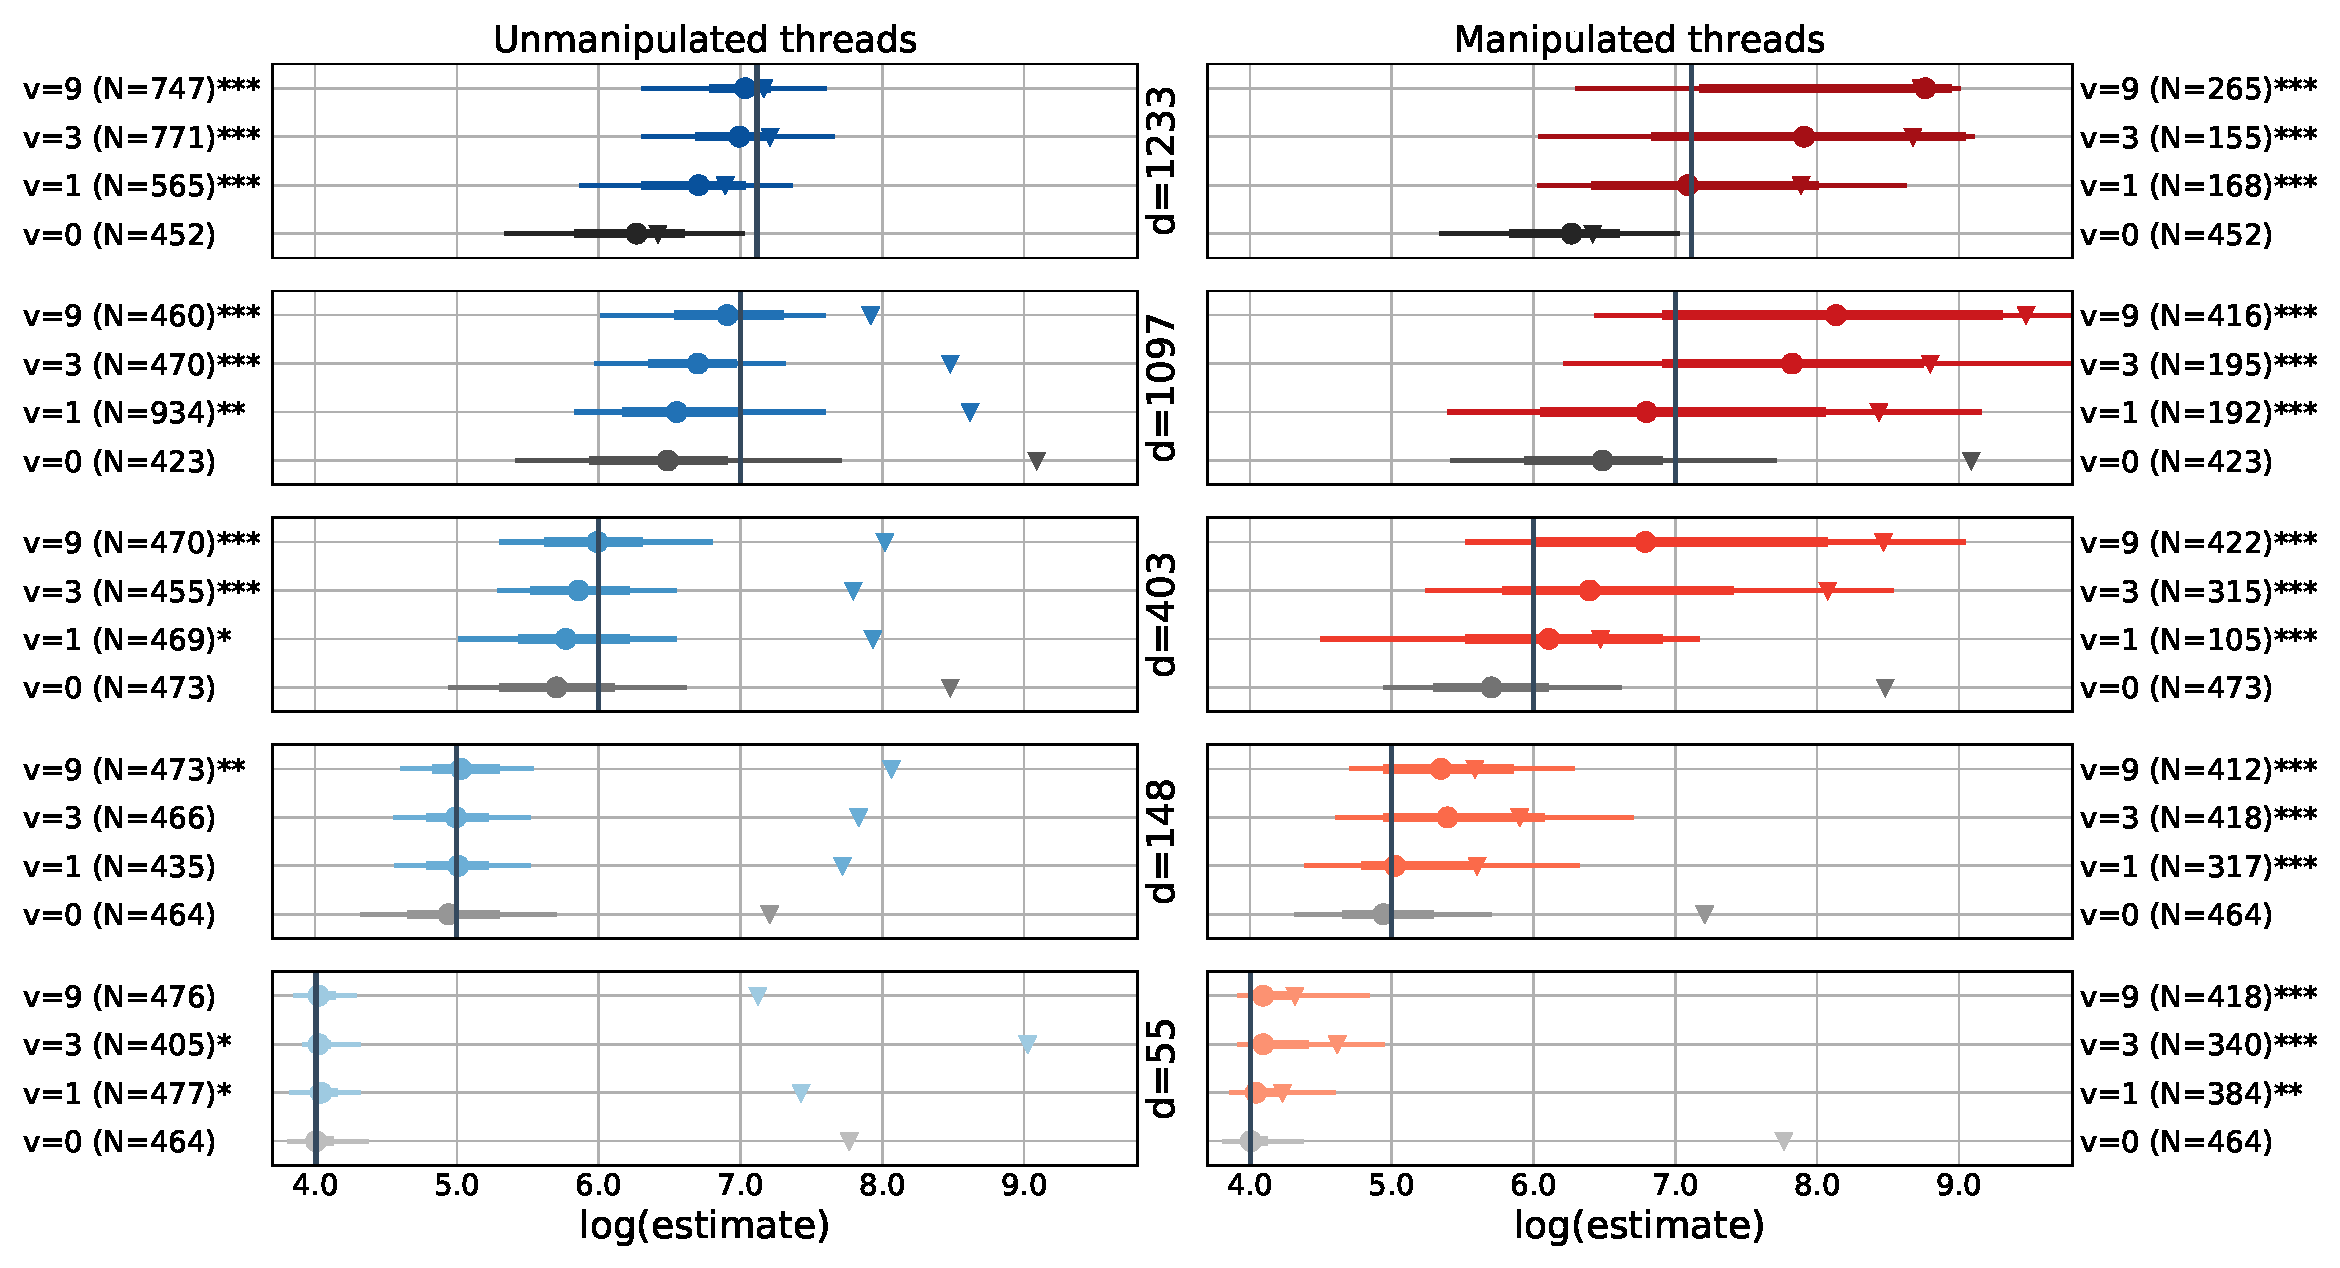
\includegraphics[width=17.4cm,height=9.5cm]{../plots/fig1max.png}
\caption{\textbf{Left:} Summary statistics of $d \times v$ treatments with a total of 10.348 magnitude estimates of either the number of dots in an image, $d \in \{55,148,403,1097\}$, or the weight of an ox, $d \in \{1233\}$, while being able to see $v \in \{0,1,3,9\}$ preceding estimates (light colors for low $d$ and dark colors for high $d$, greys show the controls). Estimates are log-transformed. Large circles indicate medians, triangles indicate arithmetic means, thick lines show interquartile ranges, thin lines show interdecile ranges, vertical black lines show the true value, and stars indicate significance levels compared to the control treatment with $v=0$ (Wilcoxon-Mann-Whitney test). No outliers were removed, making the arithmetic means strongly right skewed. \textbf{Right:} Summary statistics of $d \times v$ treatments with a total of 4.589 additional magnitude estimates, where participants do not see the preceding estimates but the $v \in \{1,3,9\}$ \textit{highest} estimates made so far. The controls, $v=0$, are the same as on the left hand side.}\label{fig:1}
\end{figure*}

\subsection*{Unmanipulated threads}
As soon as participants can see preceding estimates, accuracy improves substantially in the more difficult tasks, see the horizontal boxplots on the left hand side of figure \ref{fig:1}. The larger the view count $v$, the more accurate the median (circles) becomes. Arithmetic means (triangles) however quickly tend to overestimate the true value because free response elicitation of absolute values creates right-skewed, approximately log-normal distributions with a long tail, which inflate the means.\footnote{due to the outliers, means become highly uninformative. Even when defining a cut-off for outliers, such as an error rate of 10, would still make the arithmetic means right skewed. Galton disliked the use of the mean for this very reason as it “would give a voting power to ‘cranks’ in proportion to their crankiness” \cite{galton1907vox}. While it is still debated \cite{kao2018counteracting} which measure is best suited to aggregate social information, we focus on the median: The median is easy to interpret, is robust against outliers, and best expresses the opinion of the crowd since the majority of participants in the thread deems every other estimate as too high or too low. See also the Appendix for a discussion of outliers.} The interquartile and interdecile ranges show how high difficulty, $d$, leads to higher diversity (i.e. variation) in the dots-experiments, while higher view-counts, $v$, tend to reduce variation when $d$ is fixed, although not always.

\subsection*{Manipulated threads}
The right hand side of figure \ref{fig:1} shows the equivalent results for manipulated threads. As before, participants are relatively unaffected by social information when difficulty is low. For higher $d$'s estimates become increasingly biased towards the inflated estimates seen. In fact, we were able to create threads in which a majority of participants estimated the ox to weigth more than 6000 kilo. At points where the seen estimates became very high there were also plenty of people who started to ignore the estimates shown, especially when those estimates were ridiculously high, resulting in two branches of estimates: those showing herd behaviour by follow the previous estimates and those ignoring them, see appendix figs 6 \& 7. This lead naturally to a very high variance. Also note that for v=1, the median of the manipulated threads are often very close to the truth, because the manipulation seems to have just about the rigth size to compensate for the depressed estimates in the controls.

\begin{figure}
\centering
\includegraphics[width=1\linewidth]{../plots/fig2max.png}
\caption{\textbf{A}: In unmanipulated threads collective errors - i.e. the error of thread medians ($|truth-median|/truth$) as a function of $v$ - drop substantially in complex tasks with a high view counts (high $d$ and high $v$). For low task complexities ($d=55$, $d=148$) collective errors are small and independent of $v$. Confidence intervals (95\%) are show in error bars. \textbf{B}: In manipulated threads, collective errors increase dramatically in complex tasks with high view counts. The large error bars (95\% CI) indicate that a large fraction of participants make very high estimates. \text{C}: Median individual error (median of $|truth-estimates|/truth$) in the upper row and mean individual error (mean of $|truth-estimates|/truth$) in the lower row as a function of $v$. 95\% confidence intervals of the median/mean errors are shown as error bars. Averages (red lines) shows a general decline with increasing $v$, indicating that participants become more accurate when seeing more estimates. (\textbf{C}) Fraction of participants better than the median/mean of their thread with 95\% confidence intervals of the binomial proportions of better and worse participants as error bars. While the mean shows no change, there is a decrease in the fraction of participants better than the thread median, indicating an increasing wisdom of crowds-effect. This conclusion is corroborated in (\textbf{D}) showing the fraction of rewarded participants having made an estimate within 10\% of the true value. Confidence intervals of the binomial proportions of rewarded and non-rewarded participants are shown as error bars. The win rates increase mainly for the high-$d$ treatmens, giving an overall increase from ~22\% to ~27\% (red line), witnessing that participant’s benefit from social information. Outliers are removed.}\label{fig:2}
\end{figure}

the collective benefits substantially from social information when task difficulty is high. 


Fig. \ref{fig:2} shows the benefits of social information for collective estimation accuracy (column \textit{A}), for individual estimation accuracy (column \textit{B}), and for the ‘wisdom of threads’ (column \textit{C}). The upper row of plots refer to the median as the preferred aggregate measure, while the lower row refers to the mean. Thick red lines show the average error reduction across the tasks $d$ for increasing view counts $v$, pointing to improved collective as well as individual performance. In column \textit{D} we plot the fraction of participants within 10\% of the truth, confirming that on average participants benefit from social information. In contrast to \cite{lorenz2011social} and in concert with \cite{becker2017network, farrell2011social} this supports the claim that crowds indeed may become wise under social influence, even though wiser individuals give the aggregate wisdom of crowds measure a tougher baseline to compete against. Thus, the first main result of this article is that seeing preceding opinions in a simple estimation thread aids individual decision-making as well as the wisdom of crowds.

\subsection*{Social Influence Score}
Since individual accuracy improves with increasing samples of social information (i.e. with increasing $v$, cf. Fig. \ref{fig:2}\textit{B}), the relative accuracy of estimates compared to sample means must improve as well (SI Appendix, Fig. S4). It is not clear, however, how individuals are able to put more weight on those estimates that are closer to the true value than on estimates that are further away. One strain of explanation \cite{becker2017network, yaniv2004receiving, madirolas2015improving} suggests that individuals who are more correct are also less prone to social information, i.e. the ‘self-weight’ of their personal opinion is higher than the self-weight of others. In order to test this empirically, experiments are typically partitioned into several rounds, first by eliciting an independent estimate followed by the provision of social information, after which elicitation is repeated. This procedure makes it possible to quantify the ‘weight’ each participant put on their own opinion relative to the weight they put on the opinion of others. 

In real life it is seldomly possible to ask participants to repeat their estimates and measure their self-weight. Instead, we simply approximate the social influence of an estimate as being inversely proportional to its relative distances to the succeeding $v$ estimates. Take for instance a situation in which a participant can see $v=3$ preceding estimates: if one of the three preceding estimates is much closer to the participants’ chosen number than the two others, this ‘nearest preceding estimate’ naturally has a larger weight (‘influence’) on the participants' final estimate than the two others seen. On the other hand, if all three preceding estimates are equally far away from (or equally close to) the participants' chosen number, they all have the same weight on the final chosen number. Fig. \ref{fig:3} shows the minimum spanning tree of a thread with $d=403$ and $v=3$, in which the colors of the estimates (dots) indicate the resulting hierarchy of social influence as calculated by the relative proximity to $v$ succeeding estimates.

\begin{figure}%[tbhp]
\centering
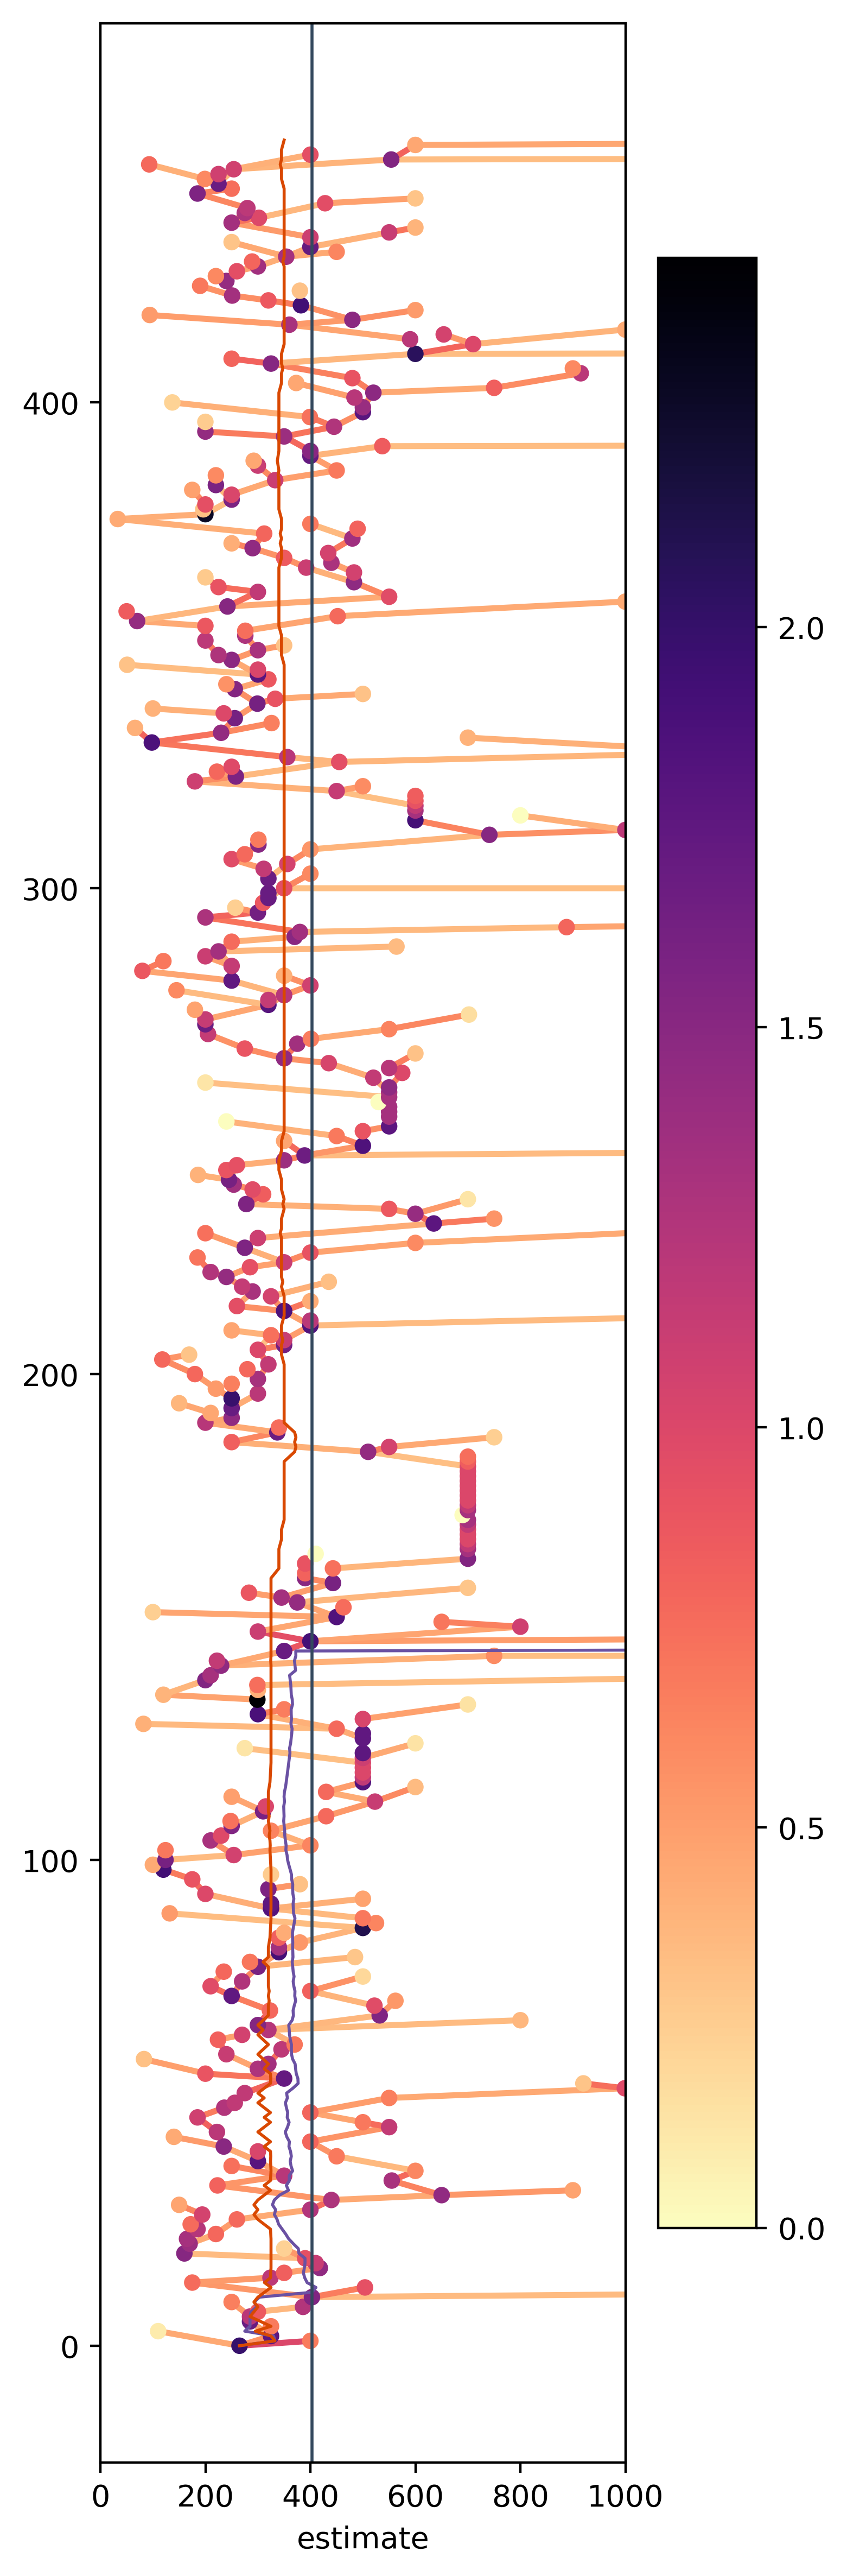
\includegraphics[width=.4\linewidth]{C:/Users/hjl161/Documents/Papers/WoT_github/plots/fig3.png}
\caption{Minimum spanning tree for a thread with $d=403$ and $v=3$ (thread position on y-axis, estimates on x-axis). Line colors indicate the relative weight $w_(r,r-k)$ of the nearest estimate observed, and dot colors specify the total social influence score $s_r$ by participant $r$ upon subsequent estimates as calculated in the main text. The black line shows the true number of dots, the blue line shows the running average (which disappears to the right on position $\tilde 140$ due to an outlier), and red line shows the running median. Four instances of short term herd behavior are observed at positions around 120, 175, 260 and 310. No outliers were removed.}
\label{fig:3}
\end{figure}

We formalize this idea by indexing participants by $r \in {1,2,...,N}$, and call their estimate $x_r$. Each $x_r$ has $d_{r,v} = (d_{r, r-1}, ..., d_{r, r-v})$ distances to the previous estimates seen, i.e. $d_{r, r-k} = |x_r-x_{r-k}|$, where $k \in \{1,...,v\}$ and $v$ is the view count. We then call the inverse of the distance between two estimates $x_r$ and $x_{r-k}$ the \textit{relative weight}, $w_{r,r-k}$, given by participant $r$ to the estimate by a preceding participant $r-k$ such that 

$$w_{r,r-k}=\frac{1}{N_rd_{r,r-k}},$$
where $N_r = \sum_{k=1}^v \frac{1}{d_{r,r-k}}$ is a normalization securing that the total weight $W_r = \sum_{k=1}^v w_{r,r-k} = 1$. The relative \textit{social influence score} $s_r$ of an estimate by participant $r$ is then given as the sum of all relative weights attributed to $x_r$ by succeeding participants who have seen it. 

$$s_r = \sum_{k=1}^v w_{r+k, r}.$$
Having calculated a social influence score $s_r$ for all estimates, we partition individual estimates into those with a higher than median social influence, called ‘high-influencers’, and those estimates with a lower than median social influence, called ‘low-influencers’. Plotting the mean relative percentage error for the high-influencers and low-influencers respectively across treatments in Fig. \ref{fig:4} reveals that high-influencers consistently are 10-40\% more correct than the low-influencers. Fig. \ref{fig:4} thus suggests that participants put more weight on estimates that are more correct, independent of any self-weight. 

\begin{figure}%[tbhp]
\centering
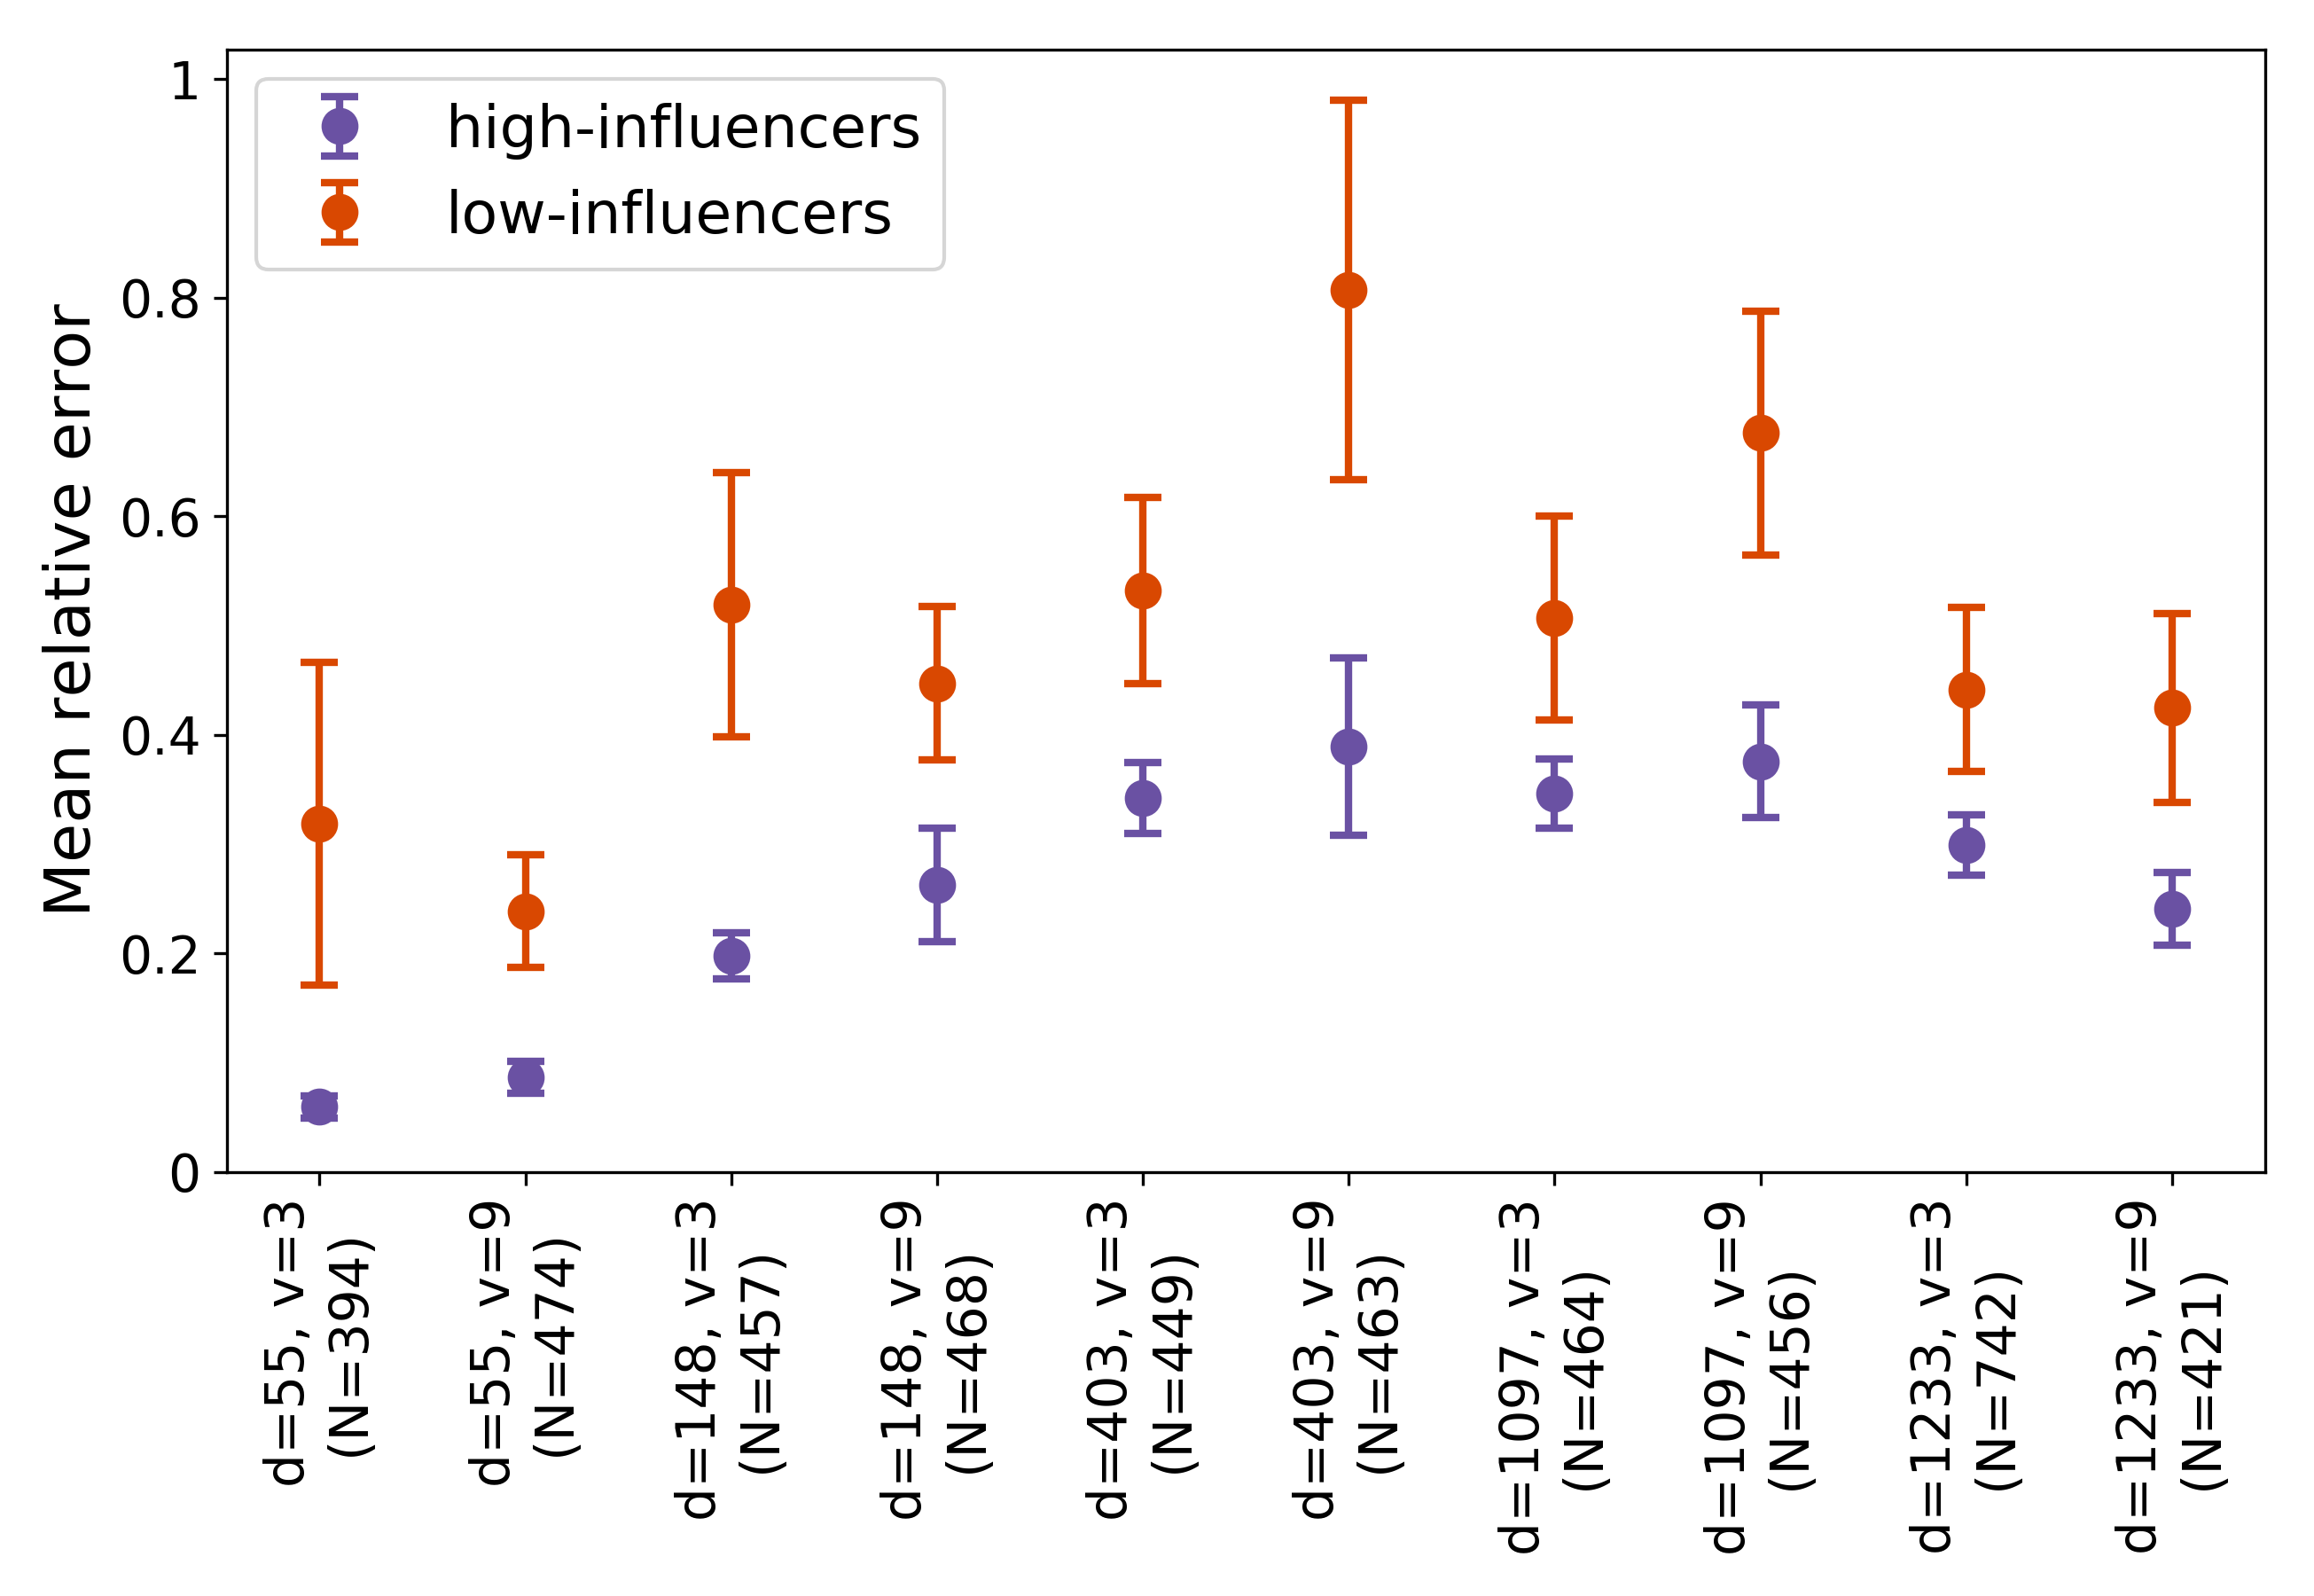
\includegraphics[width=1\linewidth]{C:/Users/hjl161/Documents/Papers/WoT_github/plots/fig4.png}
\caption{Participants who are more accurate are also more influential. High-influencers (purple) are on average 23\% less wrong than low-influencers (red), indicating a beneficial effect of social influence. Error bars show the 95\% two-sided confidence intervals for weighted means assuming normality of errors. Outliers are excluded only after social influence scores are calculated.}\label{fig:4}
\end{figure}

One must be careful when interpreting the result. The most influential estimates are typically those several successors choose as being their nearest predecessor. When inspecting the minimum spanning tree in Fig. \ref{fig:3}, it is clear that such branching points (the forks in the tree) are more centralized in comparison to the outer estimates. This suggests that the greater accuracy of high-influencers may be due to central limit effects of participants averaging the estimates they can see (their sample), rather than to an ability to endorse estimates that are more accurate. We test this hypothesis by simulating a ‘naïve social learning’ model of participants’ decision-making process, assuming that participants aggregate social and personal information evenly \cite{degroot1974reaching, golub2010naive}. Simulating such a model (see the Materials and Models section and the SI Appendix) shows that medians indeed converge towards the means for increasing $v$ (Fig. S8), indicating that at least a partial reason for the wiser threads is due to central limit effects of participants choosing an intermediate estimate. But the simulations also show no significant differences in error between high- and low-influencers (Fig. S9). This demonstrates that individual sample aggregation does not explain the increasing arithmetic means in the experiments, nor does it explain the large differences in accuracy between high- and low-influencers found in Fig. \ref{fig:4}. We may therefore conclude that participants in a thread indeed are able to find and to follow estimates that are more accurate. The second main result of this article is thus that in addition to a wisdom of crowds effect, high individual estimation accuracy translates into higher social influence among succeeding participants in a thread, and that this effect may compound in time, improving individual as well as thread accuracy even further (see SI Appendix and Fig. S10).

\subsection*{Herd Behavior}
The compounding effect of the increasing individual accuracy may easily be broken due to the high variance of estimates. But it may also be amplified by herd behavior. The minimum spanning tree in Fig. \ref{fig:3} shows four instances of herd behavior at positions $\sim 120$, $\sim 175$, $\sim 260$ and $\sim 310$. In the dots-experiments, herd behavior is rare (typically 1-5 instances in a thread of length 4-500). In the ox-experiments herd behavior is much more common (see examples in SI Appendix, Figs. S6-S7). One possible reason for frequent herd behaviors as suggested by \cite{navajas2018diversity} may be that participants are much more uncertain about their ability to estimate cattle weight compared to their ability to estimate dots on a screen. A high degree of uncertainty - or even an acceptance of cluelessness - may prompt participants to copy previous estimates rather than to make independent estimates by themselves. 

Let us look at threads with $v=9$ visible preceding estimates. One way to measure herd behavior is to count the number of participants copying predecessor estimates or being substantially close to them. Plotting in Fig. \ref{fig:5} the cumulative distribution of such copycats in terms of their percentual distance, $p$, to one or more preceding estimates shows the extend of such herd behavior and associated bandwagoning. For $p=0$, estimates are exact copies of at least one of the nine preceding estimates. For higher $p$, estimates differ by maximally $p$ percent. As may be seen in Fig. \ref{fig:5}\textit{A}, the frequency of emulating at least one preceding estimate is quite large in the ox-experiments (red) compared to the dots-experiments (purples). It turns out that herd behavior is beneficial in difficult tasks: the closer an estimate is to one or more estimates seen, the higher is the probability to win the bonus. As shown in Fig. \ref{fig:5}\textit{B}, all average relative win rates up to $p=10\%$ of copycats in threads with $d=1097$ and $d=1233$ are higher than 1, demonstrating that people can increase their win rate on average when they emulate each other. 

A bandwagon effect is observed as well, but only in the ox-experiment: Bandwagoning occurs when the rate of herd behavior increases with the number of copycats seen. Fig. \ref{fig:5}\textit{C} shows bandwagoning in the ox-experiment: when the number of identical estimates in a sample has reached 3, the rate of herd behavior increases fast, although with large error bars due to the scarcity of long bandwagons. This demonstrates that while participants in the ox-experiment are very keen to jump on the bandwagon, participants in the dots-experiments are more inclined to make up their own mind. The third and final main result of this paper is therefore that herd behavior may to amplify the positive effects of high-influencers having a higher accuracy on average. However, the prevalence of herd behavior depends strongly on the question asked, and the effects may easily become detrimental if the high-influencers are less correct.

\begin{SCfigure*}[\sidecaptionrelwidth][t]
\centering
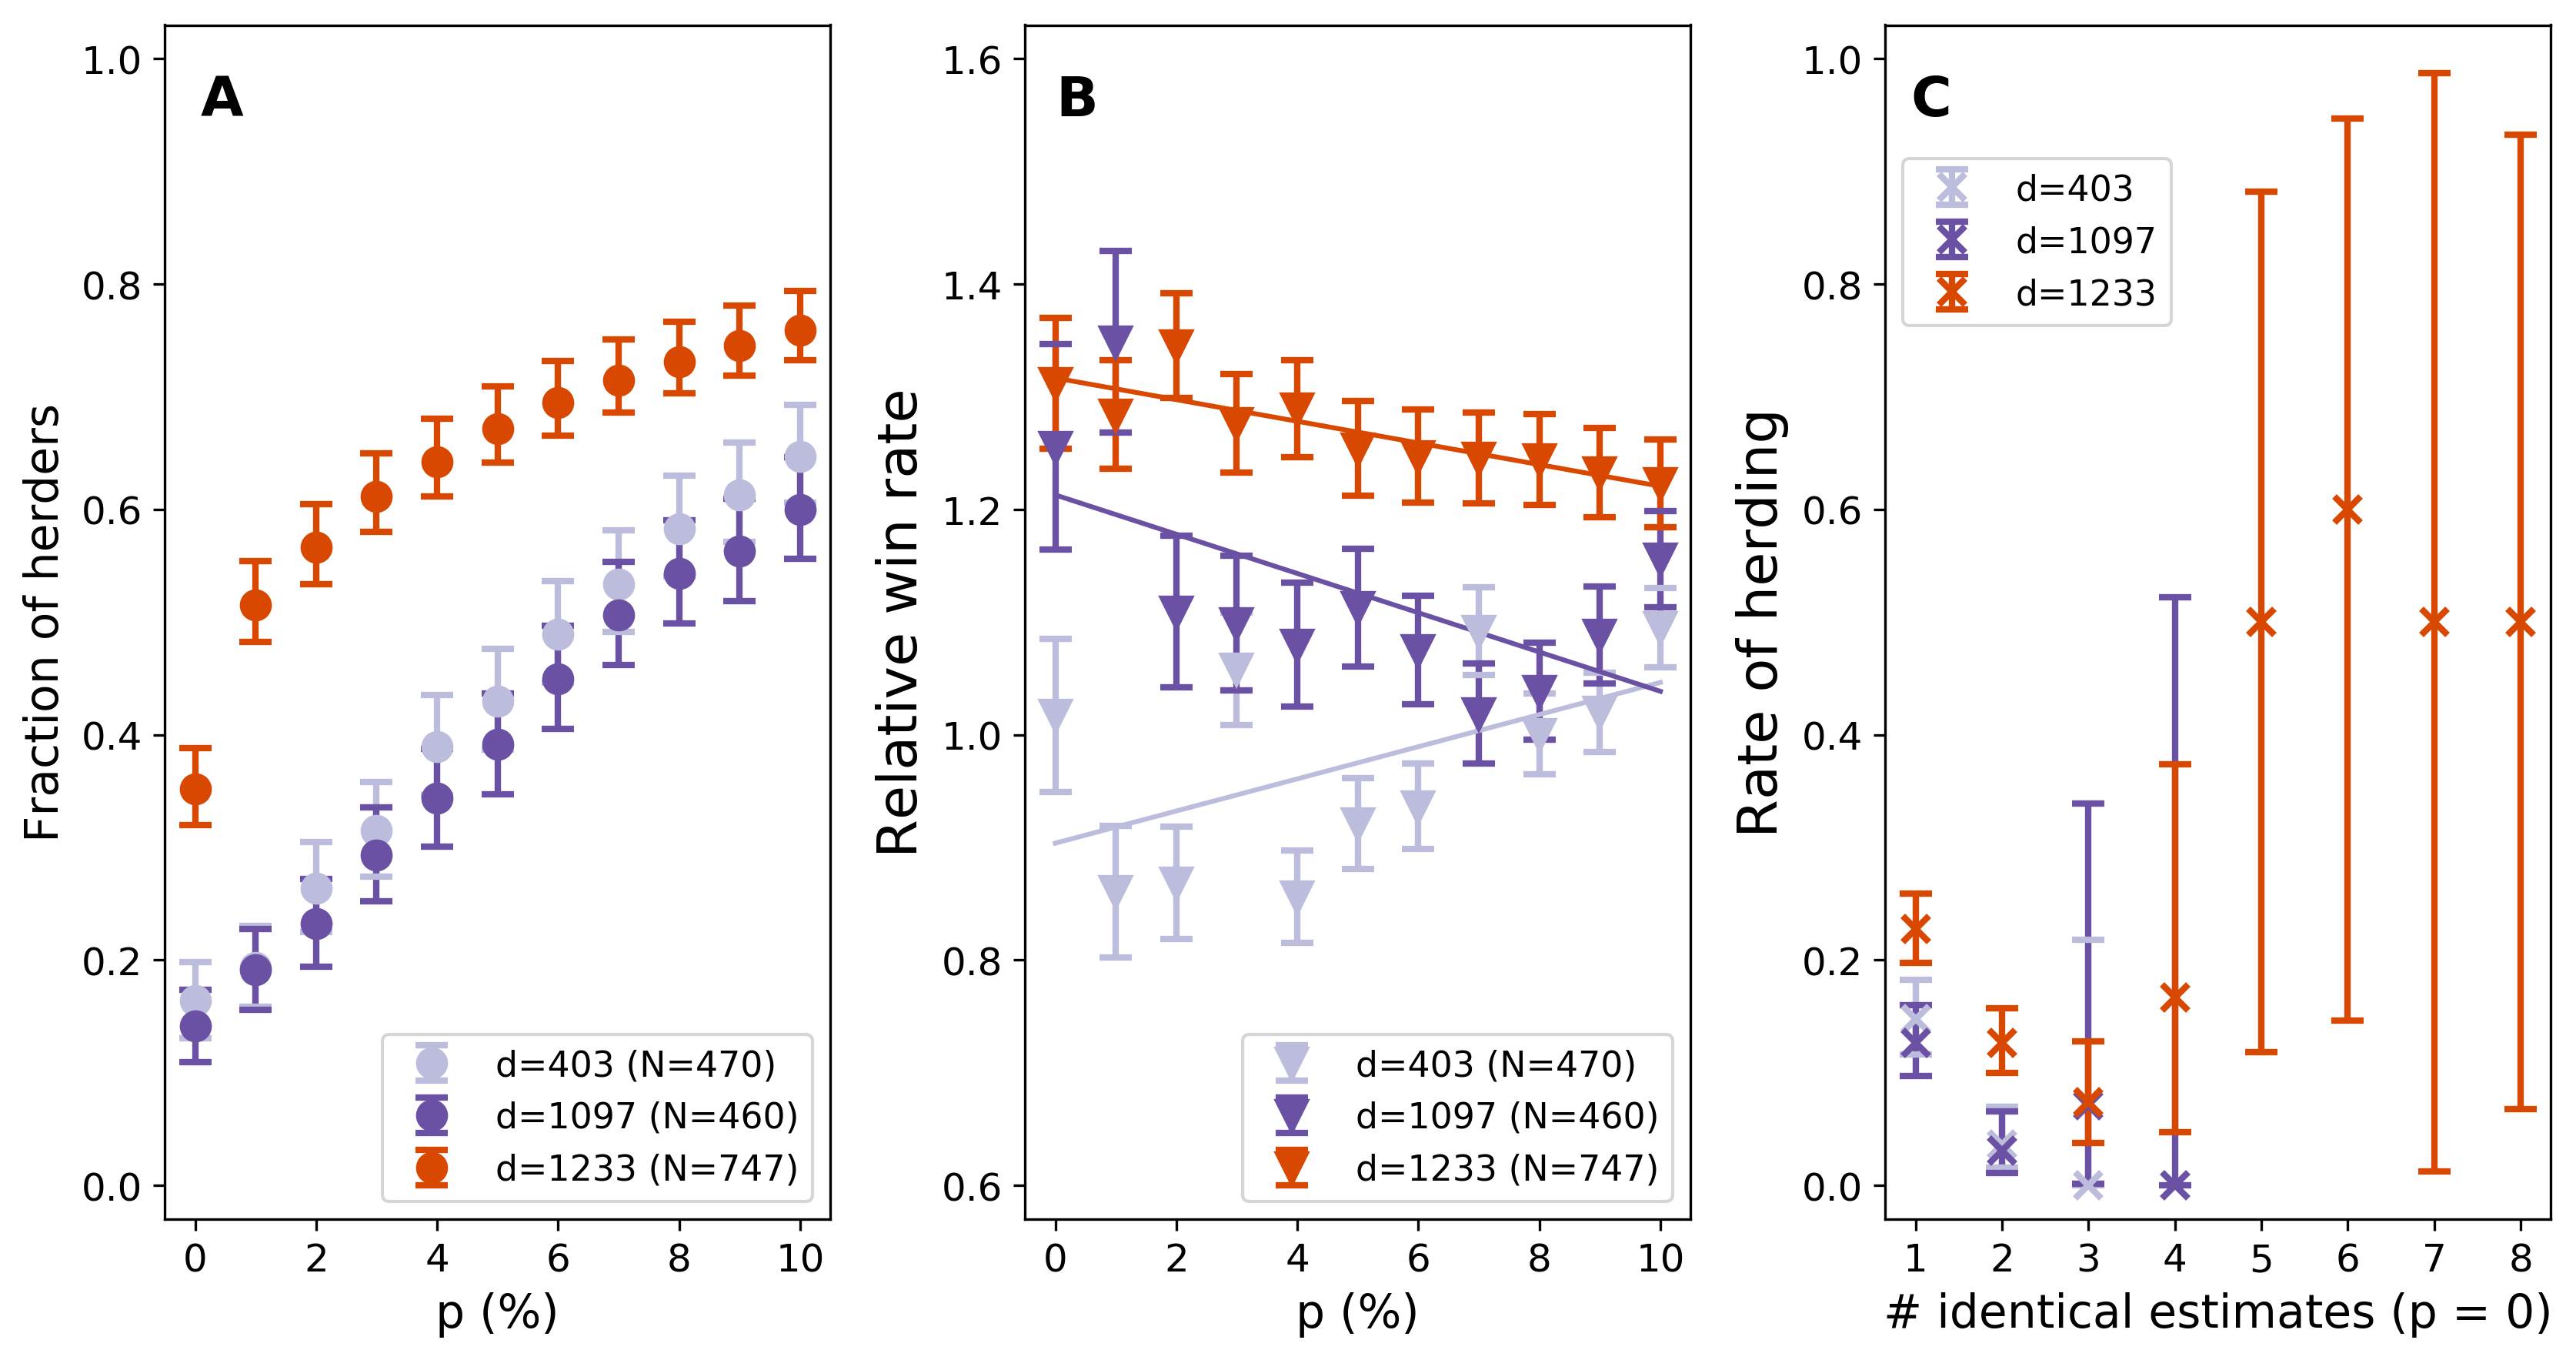
\includegraphics[width=11.4cm,height=6cm]{C:/Users/hjl161/Documents/Papers/WoT_github/plots/fig5.png}
\caption{Herd behavior and bandwagoning in threads with $v=9$. (\textbf{A}) The cumulative fraction of copycats having made estimates, which differ with maximally $p$ percent to at least one other preceding estimate in their sample. (\textbf{B}) Average win rate of copycats relative to the average win rate of all participants in a thread. Straight lines indicate the best linear fit. (\textbf{C}) A bandwagon effect is observed when the rate of herd behavior increases as a function of the number of preceding copycats, which in the ox-experiments (red) occurs for bandwagons with more than three identical estimates. However, error bars (Clopper-Pearson 95\% confidence intervals of the binomial proportions) indicate a high degree of uncertainty due to the low number of long bandwagons. There are no bandwagons with more than 3 participants when $d=403$, no bandwagons with more than 4 participants when $d=1097$ and no bandwagons with more than 8 participants when $d=1233$, respectively. No outliers are removed.}\label{fig:5}
\end{SCfigure*}

\section*{Discussion}
In the original wisdom of crowds experiment by Francis Galton, people estimated the weight of a “fat” slaughtered ox \cite{galton1907vox}. A multitude of formal and informal studies have subsequently tried to replicate Galton’s findings by using various other items, from coins and jelly beans to stock prizes and best movie nominations. This has happened even though researchers were quick to point out that the social context of such experiments, the attributes of the items such as their numerical magnitude \cite{izard2008calibrating, krueger1982single}, their extremeness and complexity \cite{nash2014curious, taleb2009errors}, as well as the expertise of the participants \cite{perry1907ballot}, are important factors to consider. 

The differences in the results of our dot-experiments and our experiment with an even stouter ox show that item attributes indeed matter. Estimating dots on a screen may or may not require as much expertise as estimating the stoutness of cattle, but the observed differences in the levels of herd behavior at least indicate that participants use different strategies when estimating different things. What does not differ, however, is a systematic underestimation bias of large numbers and a rapid improvement in individual as well as in collective accuracy when the number of visible preceding estimates is increased. The social influence measure developed in this paper is based on the assumption that proximity equates influence, which in turn establishes a natural hierarchy of influencers in a thread. Reassuringly, high-influencers turn out to be more accurate in their estimates than low-influencers across all treatment conditions. This means that the social information contained in a thread in fact helps people to calibrate their own decision-making process, even if the information may be wrong. Concerns about gullibility and correlation of judgment errors may thus be less of an evil compared to the positive effects of seeing honest opinions from other people in a thread.

Our work also gives credence to some of the conclusions drawn by social learning models, which show that groups of naïve agents can become wise under certain conditions such as high dispersion of social information \cite{golub2010naive} and decentralized communication networks \cite{becker2017network}. It remains to be seen, however, how collective and individual accuracy performs in more realistic settings. Many existing online discussion threads attach additional social information to posted comments, such as counters of ‘likes’ and sub-threaded conversations. Others carry tags of seniority or expertise, and still other threads are ranked, filtered, or manipulated in various ways. Such alterations to the basic cascade structure of a thread significantly change the topology of the communication network and has largely unknown consequences for the individual decision-making process as well as for the collective performance. These are potential directions for future work.

\matmethods{\subsection*{Experimental design and data collection} Controlled experiments of thread dynamics are rare in the research literature due to the difficulties in keeping a large number of participants in a queue. We designed our experiment along the same lines as the classical information cascade experiments by Anderson and Holt \cite{anderson1997information}. While such a design is not very feasible in normal laboratory conditions (at least for threads with several hundred participants), it is well suited for online labor markets and crowdsourcing platforms such as Amazon Mechanical Turk (AMT, see SI Appendix for further discussions of the pro and cons of AMT). We thus recruited participants from AMT to make a total of 10.808 magnitude estimations in various threads containing either an image of a certain number of dots ($d \in \{55,148,403,1097\}$) or an image of an ox ($d=1233$). After accepting our ‘HIT’ (‘human intelligence task’) and providing informed consent, participants waited in a ‘waiting room’ until the ‘choice room’ became available. When entering the choice room participants could see an image d together with $v \in \{0,1,3,9\}$ estimates made by previous participants. After making an estimate, participants were thanked and paid a participation fee of \$0.10 and bonus of \$1 if their estimate was within 10\% of the true number. The average time used was less than two minutes, see SI Appendix for screenshots and more detailed descriptions of the design and setup.
\subsection*{Outliers} We did set the minimum and maximum values submittable to be 10 and 1 million respectively. We however knew that our experiments still would be vulnerable to the dangers of free-response elicitation: 127 participants had an error rate above 10, and out of those, 62 participants had an error rate above 100. We therefore chose to trim our data when reporting aggregates. Using Tukey’s 1.5 IQR rule \cite{tukey1977exploratory} would be too exclusive however, because our distributions are not normal and because it has been previously reported that participants frequently make estimates with an error rate of 4 or more \cite{izard2008calibrating, kao2018counteracting, indow1977scaling}. The upper bound is therefore chosen to be any estimate above an error rate of 10, so that $|x_r-truth|/truth <10$, where $x_r$ is the estimate by participant $r$. We also use a lower bound of $truth/10$, due some initial reports of early timeouts and not being able to see the form input on mobile devices (see SI Appendix, section “AMT Settings”). In total, these bounds remove 254 (2.4 \%) estimates from the reported aggregate data. 
\subsection*{Simulation model} An important question is to understand how social learning may contribute to the wisdom of threads. In order to do so, we model the individual decision-making process in such a way that all participants calculate the average of all estimates seen including their own ‘hunch’, $e_r$, of what the correct number might be. By denoting an individual’s estimate $x_r$ with $r \in N$ individuals in a thread, we can calculate subsequent estimates according to $x_r = \frac{1}{v+1} \big(e_r + \sum_{i=1}^{v} x_{r-i}\big)$, where $e_r$ is a tentative guess (‘hunch’) without social information, $x_{r-i}$ are the estimates seen and $v$ is the view count. Simulating this model with values from the control experiment as the initial hunches and with increasing degrees of social information, $v$, shows that the median indeed will shift towards the arithmetic mean for increasing $v$ (SI Appendix, Fig. S8) due to the normalization of the sampling distribution (the median and mean of a normal distributions are the same). Importantly, calculating the social influence scores from the simulated data (SI Appendix, Fig. S9) reveals that there is no difference in the mean relative errors between the high- and low-influencers, respectively, demonstrating that the social influence scores shown in Fig.\ref{fig:4} are not due to any central limit effects of a naïve aggregation of social information. We therefore may conclude that the improvement in participants\' accuracy is due an ability to discriminate between better and worse estimates, and to calibrate their own estimate accordingly.}
\showmatmethods{} % Display the Materials and Methods section

\acknow{The experiments were implemented by Robin Engelhardt and Mikkel Birkegaard Andersen. Server infrastructure and devops was handled by Mikkel Birkegaard Andersen. The authors wish to thank Philipp Chapkovski for help with the cascade design, Rasmus Rendsvig for modeling discussions, and Ulrik Nash and Peter Norman Sørensen for their comments on an earlier draft of this paper. This research was approved by the Institutional Review Board at the University of Copenhagen and included informed consent by all participants in the study. The authors gratefully acknowledge the support provided by The Carlsberg Foundation under grant number CF 15-0212.}
\showacknow{} % Display the acknowledgments section

% Bibliography
\bibliography{bib_wot4}
\end{document}